\documentclass[a4paper,10pt]{article}
\usepackage{fullpage}
\usepackage{times}
\usepackage{hyperref}
\usepackage{graphicx}
\graphicspath{ {./images/} }

\begin{document}




\title{EDI: First Lab Report}
%Insert your name and ID inside the brackets
\author{Aiman Al Masoud - 502044}
\date{\today}

\maketitle

\begin{abstract}
The goal of this work was to determine the average daily peak time of a server, using an active monitoring technique (traceroute).
\end{abstract}

\clearpage

\setcounter{page}{1}
%Figures and tables must be cited in the text and explained in detail.

\section{Monitoring of a Server's Peak Time}
%Insert a brief introduction of your first lab experience


\subsection{Methodology and experimental setup}


Peak time was assumed to occur at around the early hours of the evening, more precisely: in the time interval from 6 PM to 11 PM. [\ref{article1}]


\maketitle
\subsubsection{Hypotheses that were formulated}



\underline{When a server is experiencing too many requests, the following things are expected to happen: }


\begin{itemize}

\item H1) Latency Surges: Because the server has to deal with a higher amount of packets per unit time, queueing is expected to happen, and the round trip time of packets sent to the server is expected to increase.

\item H2) Number of hops increases: At peak time, congestion may take place on the normally optimal routes, and thus alternative routes, which may include more hops, will be sought by the packets, increasing the average number of hops to reach the server.

\item H3) Number of dropped packages increases: Using UDP, there is no guarantee that the packets will reach the server, and if the network is congested and the server is busy, the drop rate is expected to increase.

\end{itemize}


\maketitle
\subsubsection{Experimental Setup}

A script that performs traceroute on a target IP at regular intervals (every 5 minutes) was executed on a vantage point for a whole week. Then the collected data was processed offline. The vantage point in question was a virtual machine on GCP (Google Cloud Platform). The target website was: www.google.com.

\subsection{Experimental results}
%Present and discuss the experimental results that you have obtained


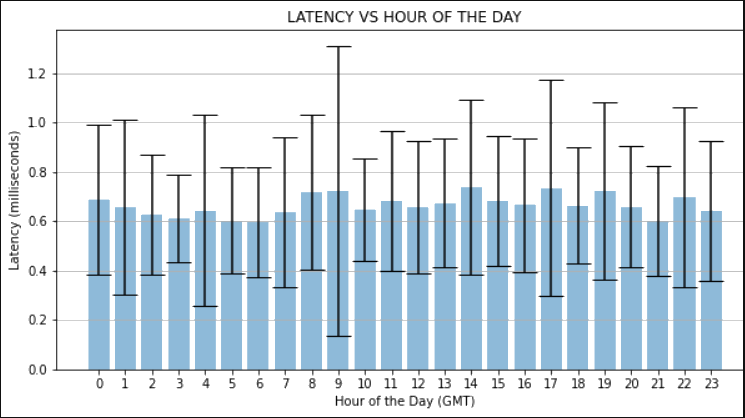
\includegraphics{latency_graph}


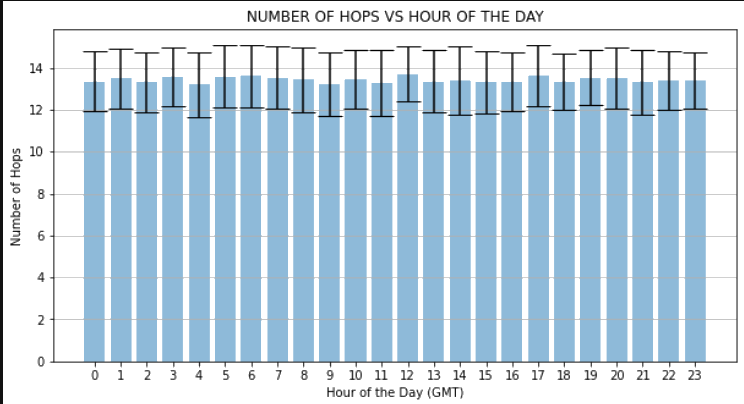
\includegraphics{hops_graph}


\begin{enumerate}

\item H1)

\item H2)

\item H3) Was found to be completely false, as the number of dropped packages stayed at a constant 0 all the time. This is most likely due to the fact that the Vantage Point and the Target servers were both owned by Google.

\end{enumerate}



\section{Insert the title of your second lab}
%Insert a brief introduction of your second lab experience
\subsection{Methodology and experimental setup}
%Discuss your methodological approach and the plan/setup of your experiments
\subsection{Experimental results}
%Present and discuss the experimental results that you have obtained
\section{Conclusion}
%Insert couple of sentences that highlight the lessons you have learnt (if any) from these lab activities.


% idk, latex needs this here for bibliography linking to work properly:
\clearpage

\section{References}


\begin{enumerate}

\item \label{article1}  \url{https://www.highspeedinternet.com/resources/why-does-my-internet-slow-down-at-night} 

\end{enumerate}







\end{document}